\documentclass[%handout,
	sans,
	12pt,
	%slidescentered,% center text on slide
	%draft,			% compile as draft version
	%notes,			% include nodes in slides
	%compress		% compress navigation bar
]{beamer}

\beamertemplatenavigationsymbolsempty

\setbeamertemplate{frametitle}
{
    \vspace*{1.5em}\insertframetitle\vspace*{-1.5em}
}

\usepackage[T1]{fontenc}
\usepackage[utf8x]{inputenc}

\usepackage{mathpazo}
\usepackage[british]{babel}
\usepackage{csquotes}

\usepackage{svg}

\newcommand{\high}[1]{{\usebeamercolor[fg]{structure} #1}}
\newcommand{\bad}[1]{\textcolor{red}{#1}}
\newcommand{\gray}[1]{\textcolor{darkgray}{#1}}
\newcommand{\black}[1]{\textcolor{black}{#1}}

\usepackage{amsmath,amssymb}
\usepackage{upgreek}
\usepackage{booktabs}
\usepackage{hyperref}
\usepackage{default}
\usepackage{graphicx}
\usepackage{colortbl}
\usepackage{url}
\usepackage{setspace}
\usepackage{wrapfig}
\usepackage{tabularx}

\setbeamertemplate{caption}[numbered]

\newcommand{\RR}{\mathbb{R}}
\newcommand{\NN}{\mathbb{N}}
\def\braces#1{[#1]}

%\definecolor{mybg}{rgb}{0.9,0.9,0.9}
\definecolor{mybg}{rgb}{1,1,1}
\setbeamercolor{background canvas}{bg=mybg}

\title{An executables specification of BDDs in Isabelle}
\author{\normalsize Max Haslbeck and Julius Michaelis}
\institute[]{\footnotesize Fakultät für Informatik\\TU München}
\date{\footnotesize 26 February 2016}

\begin{document}

\maketitle


\section{Introduction - BDDs}
\begin{frame}{Introduction - BDDs}
  \begin{center}
\begin{figure}[htbp]
  \centering
  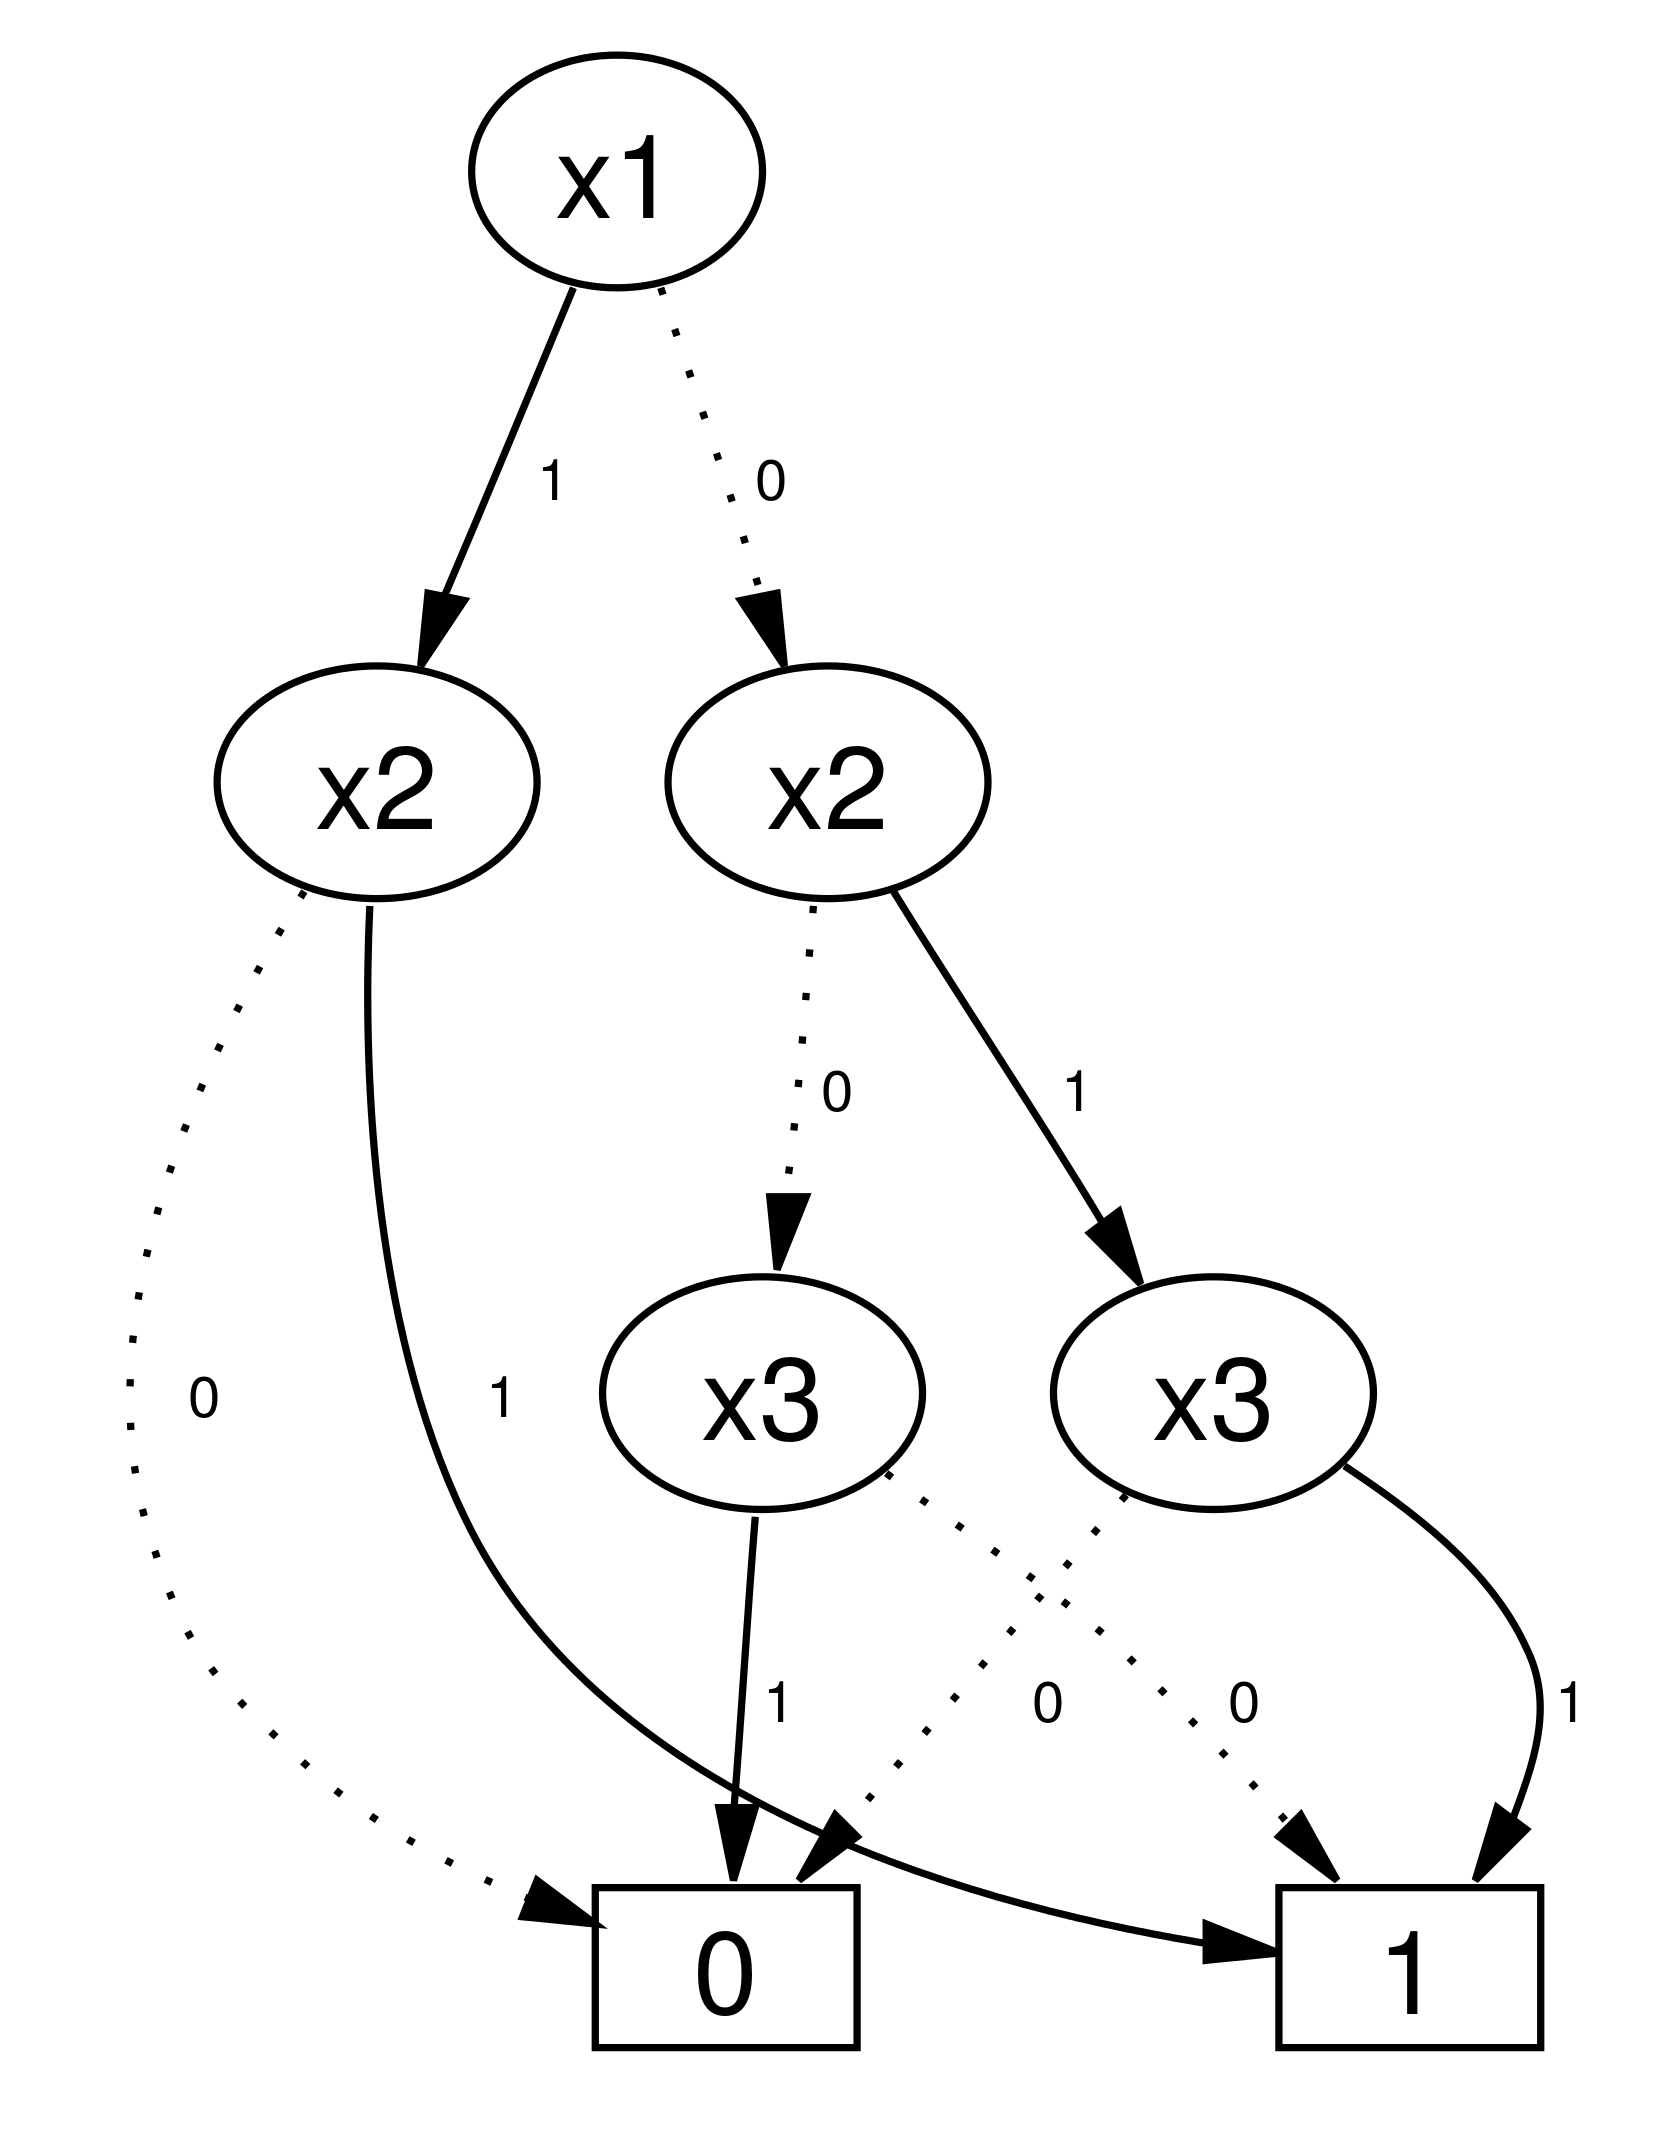
\includegraphics[height=5cm]{img/BDD_simple.png}
  \caption{BDD $(\overline{x_1} \land \overline{x_2} \land \overline{x_3}) \lor
  (x_1 \land x_2) \lor (x_2 \land x_3) $}
\end{figure}
  BDD = Binary Decision Diagram \\
  ROBDD = Reduced Ordered Binary Decision Diagram
  \end{center}
\end{frame}


\section{Formalization in Levels}

\begin{frame}{Boolean functions}

\begingroup
\addtolength{\jot}{-1mm}
{\footnotesize
\begin{flalign*}
  &\textbf{type\_synonym}\ \tau\ bf\ \textbf{=}\ (\tau \Rightarrow bool)
   \Rightarrow bool& \\[1\baselineskip]
 &    \textbf{definition}\ \textit{bf-ite}\ ::\ \tau\ bf \Rightarrow
 \tau\ bf \Rightarrow \tau\ bf \Rightarrow \tau\ bf\ \textbf{where}&  \\
 &\hskip4mm   \textit{bf-ite}\ i\ t\ e\ =\ (\lambda x.\ \text{if}\ i\ x\ \text{then}\ t\ x\
\text{else}\ e\ x)& \\[1\baselineskip]
 &    \textbf{definition}\ \textit{bf-restrict}\ ::\ \tau\ bf \Rightarrow
\tau \Rightarrow bool \Rightarrow \tau\ bf\ \textbf{where}&  \\
&\hskip4mm \textit{bf-restrict}\ f\ v\ b\ =\ (\lambda a.\ f\ (a(v := b))&
\\[1\baselineskip]
 & \textbf{lemma:}\ \textit{bf-ite}\ I\ T\ E\ =&\\
 &\phantom{\textbf{lemma:}}\ \textit{bf-ite}\ (\lambda l.\ l\ v)& \\
 &\phantom{\textbf{lemma:}\ \textit{bf-ite}}\
 (\textit{bf-ite}\ (\textit{bf-restrict}\ I\ v\ \textit{True})\
 (\textit{bf-restrict}\ T\ v\ \textit{True})& \\
 &\phantom{\textbf{lemma:}\ \textit{bf-ite}\ (\textit{bf-ite}}\
 (\textit{bf-restrict}\ E\ v\ \textit{True}))& \\
 &\phantom{\textbf{lemma:}\ \textit{bf-ite}}\
 (\textit{bf-ite}\ (\textit{bf-restrict}\ I\ v\ \textit{False})\
 (\textit{bf-restrict}\ T\ v\ \textit{False})& \\
 &\phantom{\textbf{lemma:}\ \textit{bf-ite}\ (\textit{bf-ite}}\
 (\textit{bf-restrict}\ E\ v\ \textit{False}))&
\end{flalign*}
}
\endgroup
\vspace*{-10mm}
\end{frame}


\begin{frame}{Binary Decision Trees}
\begingroup
\addtolength{\jot}{-1mm}
{\footnotesize
\begin{flalign*}
  &\textbf{datatype}\ (\tau :: \textit{linorder})\ \textit{bdt}\ \textbf{=}\ \textit{Trueif}\ |\ 
  \textit{Falseif}\ |\ IF\ \tau\ (\tau\ \textit{bdt})\ (\tau\ \textit{bdt})
  & \\[\baselineskip]
   & \textbf{definition}\ \textit{bf-bdt-rel}\ =
      \{(bf, bd).\ \textit{ro-bdt}\ bd\ \land\ \forall a.\ bf\ a =
      \textit{val-bdt}\ bd\ a\} & \\[\baselineskip]
      & \textbf{lemma:}\ (bf,bd) \in \textit{bf-bdt-rel} \Longrightarrow
                    (bf',bd') \in \textit{bf-bdt-rel}& \\
     & \phantom{lemma:}\
       \Longrightarrow  (bf = bf') \leftrightarrow (bd = bd')
 &
\end{flalign*}
}


\endgroup
\vspace*{-10mm}
\end{frame}

\begin{frame}{Binary Decision Trees}
\begin{figure}[htbp]
  \centering
  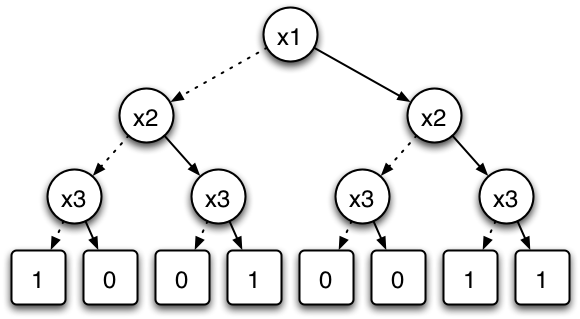
\includegraphics[height=5cm]{img/BDT.png}
  \caption{BDT $(\overline{x_1} \land \overline{x_2} \land \overline{x_3}) \lor
  (x_1 \land x_2) \lor (x_2 \land x_3) $}
\end{figure}
\end{frame}


\begin{frame}{BDDs on abstract datatypes}
  Picasso.
\end{frame}

\subsection{A concrete datatype: Pointermap}
\subsection{Towards fast execution}
\subsection{Collapsed Result}
\begin{frame}
\end{frame}
\section{Evaluation}
\begin{frame}{Benchmarks}
\end{frame}





\end{document}
